\documentclass{article}

\usepackage{amsmath,graphicx,parskip,mathrsfs,subfigure}
\usepackage{fancyhdr}
\usepackage{amsthm,amssymb}
\usepackage{setspace}
\usepackage{epstopdf}
\usepackage[left=3cm,right=3cm,top=3cm,bottom=3cm]{geometry}
\usepackage{natbib}

\pagestyle{fancy}
\lhead{Samuel Huberman}
\chead{MSE1022: Final Report}
\rhead{999157923}

\linespread{1}
\begin{document}

\section*{Introduction}

The objective of this study was to observe the effect of an interface upon phonon properties. Here, an interface is defined by enforcing a mass difference in a Lennard-Jones Argon system. Using a combination of data from molecular dynamics and lattice dynamics calculations, the linewidth of a phonon (which is inversely proportional to the phonon's lifetime) is obtained. It will be shown that this approach, in its current implementation, will not offer the insight required to infer the extent of the presence of the interface upon the lifetimes.

\section*{Theory}

\begin{figure}[ht]
\centering
\includegraphics[scale=0.5]{diatomic.png}
\caption{Diagram of a linear diatomic chain of atoms}
\end{figure}
Lattice dynamics, in its most basic form, involves solving the equations of motion of a multiple degree of freedom coupled harmonic oscillator system \cite{dove}. Recalling the equations of motion of a linear diatomic chain considering only nearest neighbour interaction ($K_1$ and $K_2$ are the respective spring constants in accordance with Hooke's Law) as shown in Figure 1
\begin{eqnarray}
	M\frac{\partial ^2 U_n}{\partial t^2}&=-K_1(U_n-u_n)-K_2(U_n-u_{n-1})\\
	m\frac{\partial ^2 u_n}{\partial t^2}&=-K_1(u_n-U_n)-K_2(u_n-U_{n+1}),
\end{eqnarray}
one recognizes that the solutions to the equations will have the periodic form
\begin{eqnarray}
	U_n&=\sum_\kappa \tilde{U_\kappa}e^{i(\pmb{\kappa} x-\omega t)}\\
	u_n&=\sum_\kappa \tilde{u_\kappa}e^{i(\pmb{\kappa} x-\omega t)}.
\end{eqnarray}
Upon the application of the proper boundary conditions (the Born-von Karman periodic boundary, where the last atom in the chain is equivalent to the first in the chain), a discrete set of allowed values of $\pmb{\kappa}$ emerges (this condition is not affected by the fact that the masses of the chain alternate; the unit cell contains the two atoms) from the restriction of physically meaningful solutions and avoiding the trivial solution
\begin{eqnarray}
	\pmb{\kappa}=\frac{2\pi m}{Na}.
\end{eqnarray}
Each $\pmb{\kappa}$ in this set corresponds to a different phonon mode. Noting that the values of the equilibrium positions of $x$ are restricted to integer values of $a$, the set of coupled ordinary differential equations can be represented in terms of an eigenvalue problem
\begin{eqnarray}
\begin{bmatrix}
  -M\omega_\kappa^2 & 0\\
  0 & -m\omega_\kappa^2\\ 
 \end{bmatrix}
\begin{bmatrix}
\tilde{U_\kappa} \\ 
\tilde{u_\kappa}
\end{bmatrix}
=
\begin{bmatrix}
  -(K_1+K_2) & K_1+K_2e^{-i\pmb{\kappa} a}\\
  -(K_1+K_2) & K_1+K_2e^{-i\pmb{\kappa} a}\\ 
 \end{bmatrix}
\begin{bmatrix}
\tilde{U_\kappa} \\ \tilde{U_\kappa}.
\end{bmatrix}
\end{eqnarray}
The eigenvalues are the square of the allowed frequencies and the eigenvectors are the allowed amplitudes for a given value of $\pmb{\kappa}$. The range of wavevectors, which operate in reciprocal space,  $\frac{-\pi}{a}\leq \pmb{\kappa}\leq\frac{\pi}{a}$ gives the first Brillouin zone. Because of the periodic nature of the lattice and hence $\pmb{\kappa}$, values outside this region may be folded back over so as to be included in the first Brillouin zone.

This 1-D case can easily be generalized to the more relevant 3-D case of a harmonic crystalline solid, where atoms have three degrees of freedom and modes are specified by wavevector $\pmb{\kappa}$ and branch $\nu$. The global solution of the displacement of atom $j$ in unit cell $l$ at time $t$ is given by a superposition of all possible solutions of the equations of motion
\begin{eqnarray}
\pmb{u}(jl,t)&=\sum_{\pmb{\kappa},\nu}\pmb{U}(j,\pmb{\kappa},\nu)exp(i[\pmb{\kappa} \cdot \pmb{r}(jl)-\omega(\pmb{\kappa},\nu)t])\\
&=\frac{1}{\sqrt{Nm_j}}\sum_{\pmb{\kappa},\nu}\pmb{e}(j,\pmb{\kappa},\nu)exp(i\pmb{\kappa}\cdot\pmb{r}(jl))Q(\pmb{\kappa},\nu)
\end{eqnarray}
where $\pmb{r}(jl)$ is the equilibrium position of atom $jl$, according to the defined coordinate system. The general eigenvalue problem has the form
\begin{eqnarray}
\pmb{D}(\pmb{\kappa})\pmb{e}(\pmb{\kappa},\nu)=\omega^2_{\kappa}\pmb{e}(\pmb{\kappa},\nu)
\end{eqnarray}
where $\pmb{D}(\pmb{\kappa})$ is the dynamical matrix, containing the second order terms of the potential energy expansion. $\pmb{e}(\pmb{\kappa},\nu)$ and $\omega^2_{\kappa}$ are the eigenvector and eigenvalue, respectively. Since $\pmb{D}(\pmb{\kappa})$ is a Hermitian matrix (a consequence of the commutative property of derivatives), the eigenvectors will be orthogonal. Taking the Fourier Transform of the global solution and using this orthogonal property of the eigenvectors, the normal modes coordinates are obtained
\begin{eqnarray}
\dot{Q}(\pmb{\kappa},\nu,t)&=\frac{1}{\sqrt{N}}\sum_{jl}\sqrt{m_j}exp(-i\pmb{\kappa}\cdot\pmb{r}(jl))\pmb{e}^*(j,\pmb{\kappa},\nu)\cdot\dot{\pmb{u}}(jl,t).
\end{eqnarray}
The normal modes are the natural vibrations of the system, by which every motion can be constructed as a superposition of these modes. In essence, the normal modes provide the ability to decouple the equations of motions and treat the system as a number of independent harmonic oscillators (In operator formalism, the Hamiltonian is diagonalized). ${Q}(\pmb{\kappa},\nu,t)$ is viewed as the number (or population) of phonons of mode $\pmb{\kappa},\nu$ that exist in the system at time $t$ and $\dot{Q}(\pmb{\kappa},\nu,t)$ is the rate of change of this population. 

In a real crystal system, the interatomic potential is not harmonic and the truncation of the energy expansion and the second-order term will not recover such physical behaviour as thermal expansion or finite thermal conductivity. The anharmonic properties, while of considerable significance, remain challenging to computationally predict, in part because there does not exist a functional form for the solution to the anharmonic equations of motion. Anharmonicity in the interatomic potential manifests by perturbing the crystal's lattice constant, interrupting the perfect periodicity and thus scattering phonons. The average time between scattering events of a given mode $\pmb{\kappa},\nu$ is the lifetime $\tau_{p-p}(\pmb{\kappa}, \nu)$. As a consequence of this aharmonicity, $\dot{Q}(\pmb{\kappa},\nu,t)$ will no longer behave sinusoidally in time, but will contain an exponential term proportional to this lifetime. The objective of this work is to observe the difference between bulk phonon lifetimes and phonon lifetimes near an interface (we expect that given enough distance from the interface, the phonon lifetimes correspond to the bulk phonon lifetimes) using Normal Mode Decomposition (NMD).

\section*{Implementation}

NMD is an algorithm that combines time-dependent information from molecular dynamics and the harmonic solutions from lattice dynamics to infer the phonon lifetimes \cite{larkin}. Although this approach relies on the empirical potentials of classical MD, the complete anharmonicity is considered (other methods, like DFPT, truncate terms beyond the third order derivatives).

Using GULP to solve the eigenvalue problem from Equation 9, the eigenvectors and frequencies were determined for given set of points in the Brillouin zone. Then, by taking a series of velocity samples from the LAMMPS simulation of time interval (in signal processing terminology, this is known as lag which is symbolically represented here by $t$) an order of magnitude shorter than the inverse of the highest vibrational frequency present in the system (determined from the GULP calculation) and using Equation 10 to project the sampled velocities onto the eigenvectors, the autocorrelation of the normal modes can calculated by
\begin{equation}
C(\pmb{\kappa},\nu,t)=\lim_{T->\infty}\frac{1}{T}\int_{0}^{T}Q(\pmb{\kappa},\nu,t+t')Q(\pmb{\kappa},\nu,t')dt'.
\end{equation}
The spectral energy density (SED), from the Wiener-Khintchine theorem, is thus
\begin{equation}
C(\pmb{\kappa},\nu,\omega)=\int_{-\infty}^{\infty}C(\pmb{\kappa},\nu,t)e^{-i\omega t}dt.
\end{equation}
This is a Fourier Transform of an exponential function, which yields a Lorentzian centered at $\omega_0(\pmb{\kappa},\nu)$
\begin{equation}
C(\pmb{\kappa},\nu,\omega)=\frac{C_0(\pmb{\kappa},\nu)}{2}\frac{\Gamma(\pmb{\kappa},\nu)/\pi}{(\omega_0(\pmb{\kappa},\nu)-\omega)^2+\Gamma(\pmb{\kappa},\nu)}.
\end{equation}
The half width at half maximum of the Lorentzian is related by anharmonic lattice dynamic theory to phonon lifetime by
\begin{equation}
\tau_{p-p}(\pmb{\kappa}, \nu)=\frac{1}{2\Gamma(\pmb{\kappa},\nu)}.
\end{equation}
In order to ensure the statistical significance of the results, an averaging scheme was needed. Five MD simulations were performed, each with a different initial velocity seed. In each MD simulation, 16 sets of atomic velocities were produced. Each set of velocities consisted of 2048 subsets of atomic velocities; the lag between subsets was 32 LJ time units (in other words, velocities were sampled every 32 LJ time units for a total of 2048 samples). The power of two formulation was chosen for the sake of the fast Fourier Transform. $\dot{Q}(\pmb{\kappa},\nu,t)$ was calculated for each individual velocity subset (Equation 10) and then used as input for the correlation function (Equation 11) and SED (Equation 12) of the set. Finally the SED is averaged over the 16 sets and 5 seeds. This procedure was performed on three cases: (A) a 4 unit cell by 4 unit cell by 4 unit cell (hereby referred to as 4x4x4) domain of Lennard-Jones Argon in equilibrium at 20 K with periodic boundary conditions (B) a 32x4x4 domain of LJAr at 20K with periodic boundary conditions and (C) 32x4x4 domain of LJAr at 20K, where one half (16x4x4) is set to the unit mass of Argon and the other half is set to three times the unit mass of Argon, with periodic boundary conditions. Cases B and C are divided into 4x4x4 blocks for the post-processing steps (NMD-SED) to match the phonon modes present in Case A (see Figure 2), in an attempt to offer a mode by mode comparison (the results from Block 1 for both B and C are presented in the Results and Discussion section). 

\begin{figure}[ht]
\centering
\includegraphics[scale=0.5]{mddom1.jpg}
\caption{MD domain for interface study of 32x4x4 fcc Argon at 20K with 2048 atoms}
\label{fig:subfig1}
\end{figure}

\section*{Results and Discussion}
As the plane of the interface has a normal in the $x$ direction, it is reasonable to expect wavevectors containing some $x$ component to be affected. For simplicity, the modes at $\pmb{\kappa}=[1,0,0]$ in the BZ are examined. 
\begin{figure}[h!]
\centering
\subfigure[\small{$\pmb{\kappa}=[1,0,0]$,$\nu=$TA}]{
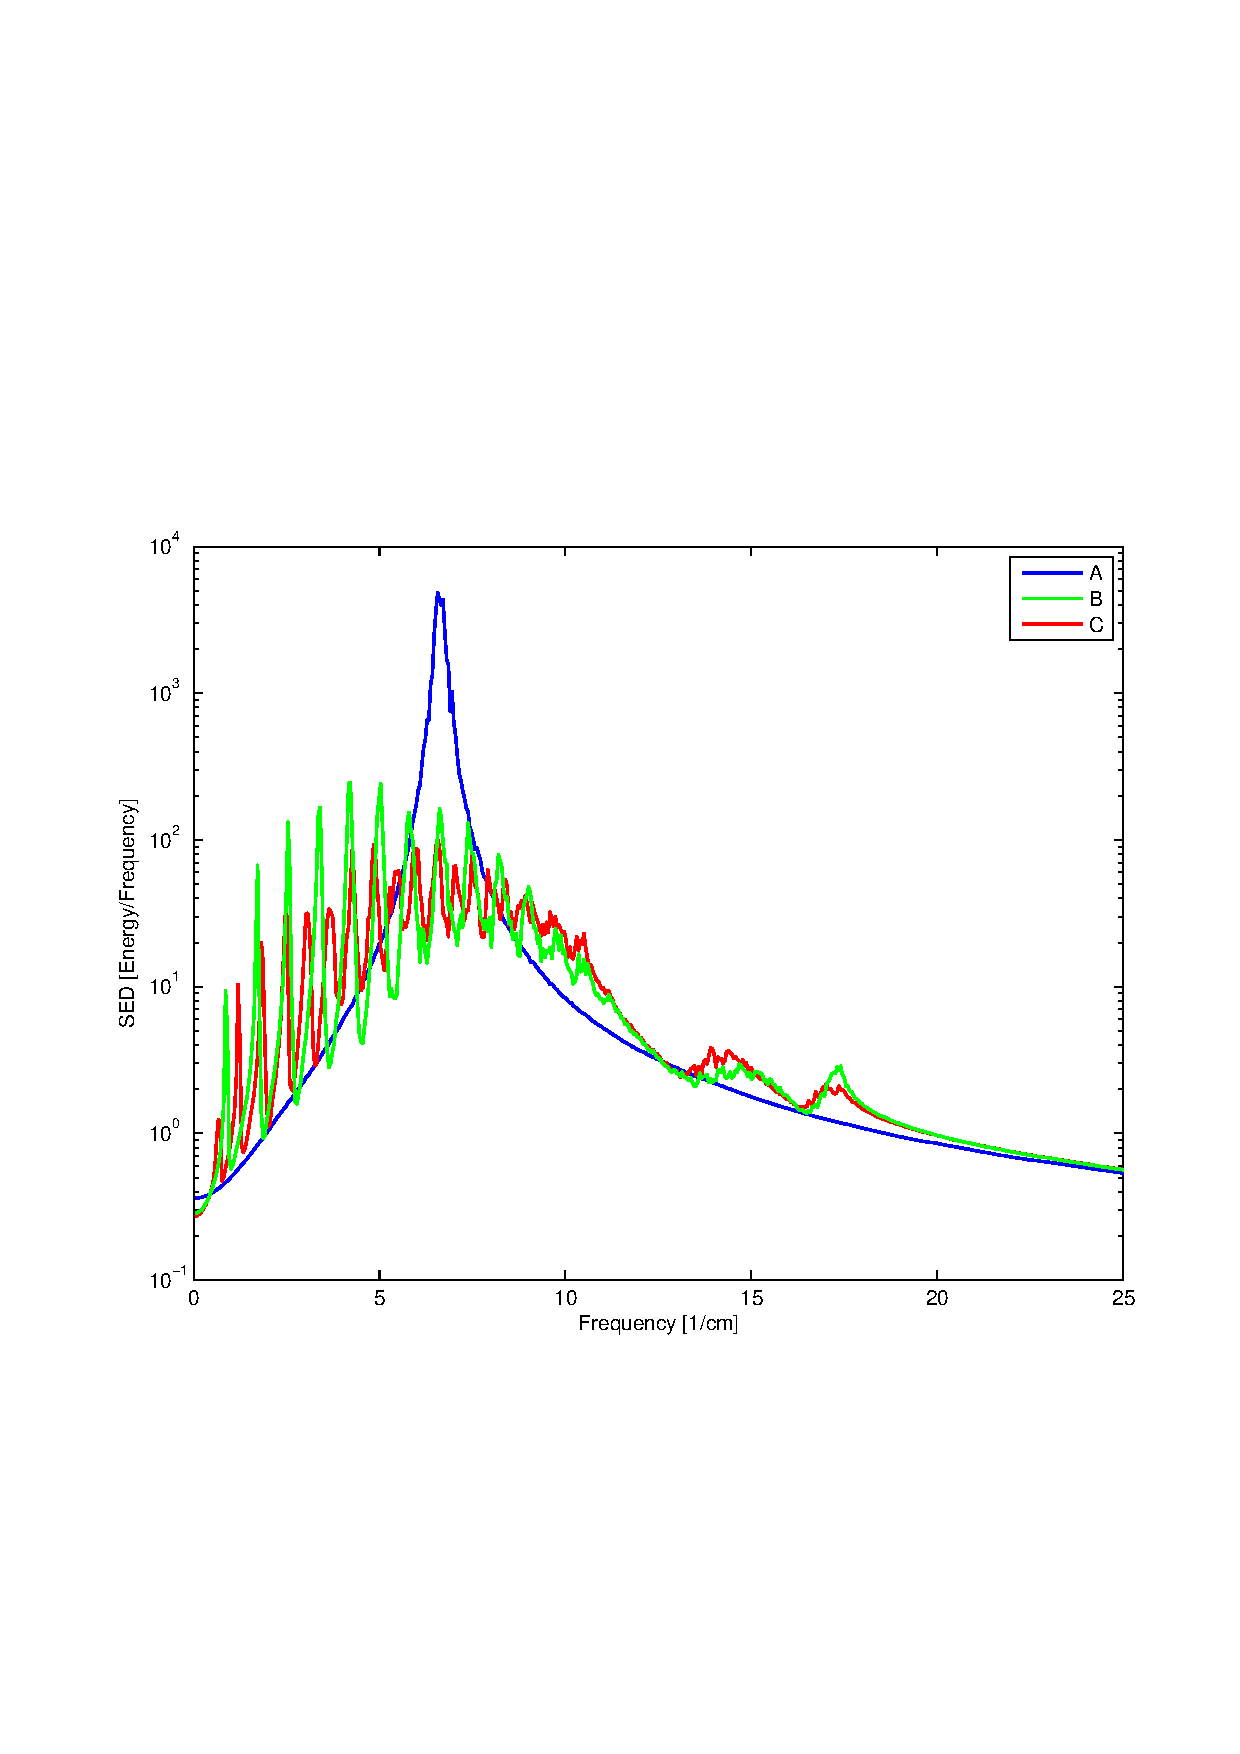
\includegraphics[scale=0.4]{peak_100_TA}
}
\subfigure[\small{$\pmb{\kappa}=[1,0,0]$,$\nu=$LA}]{
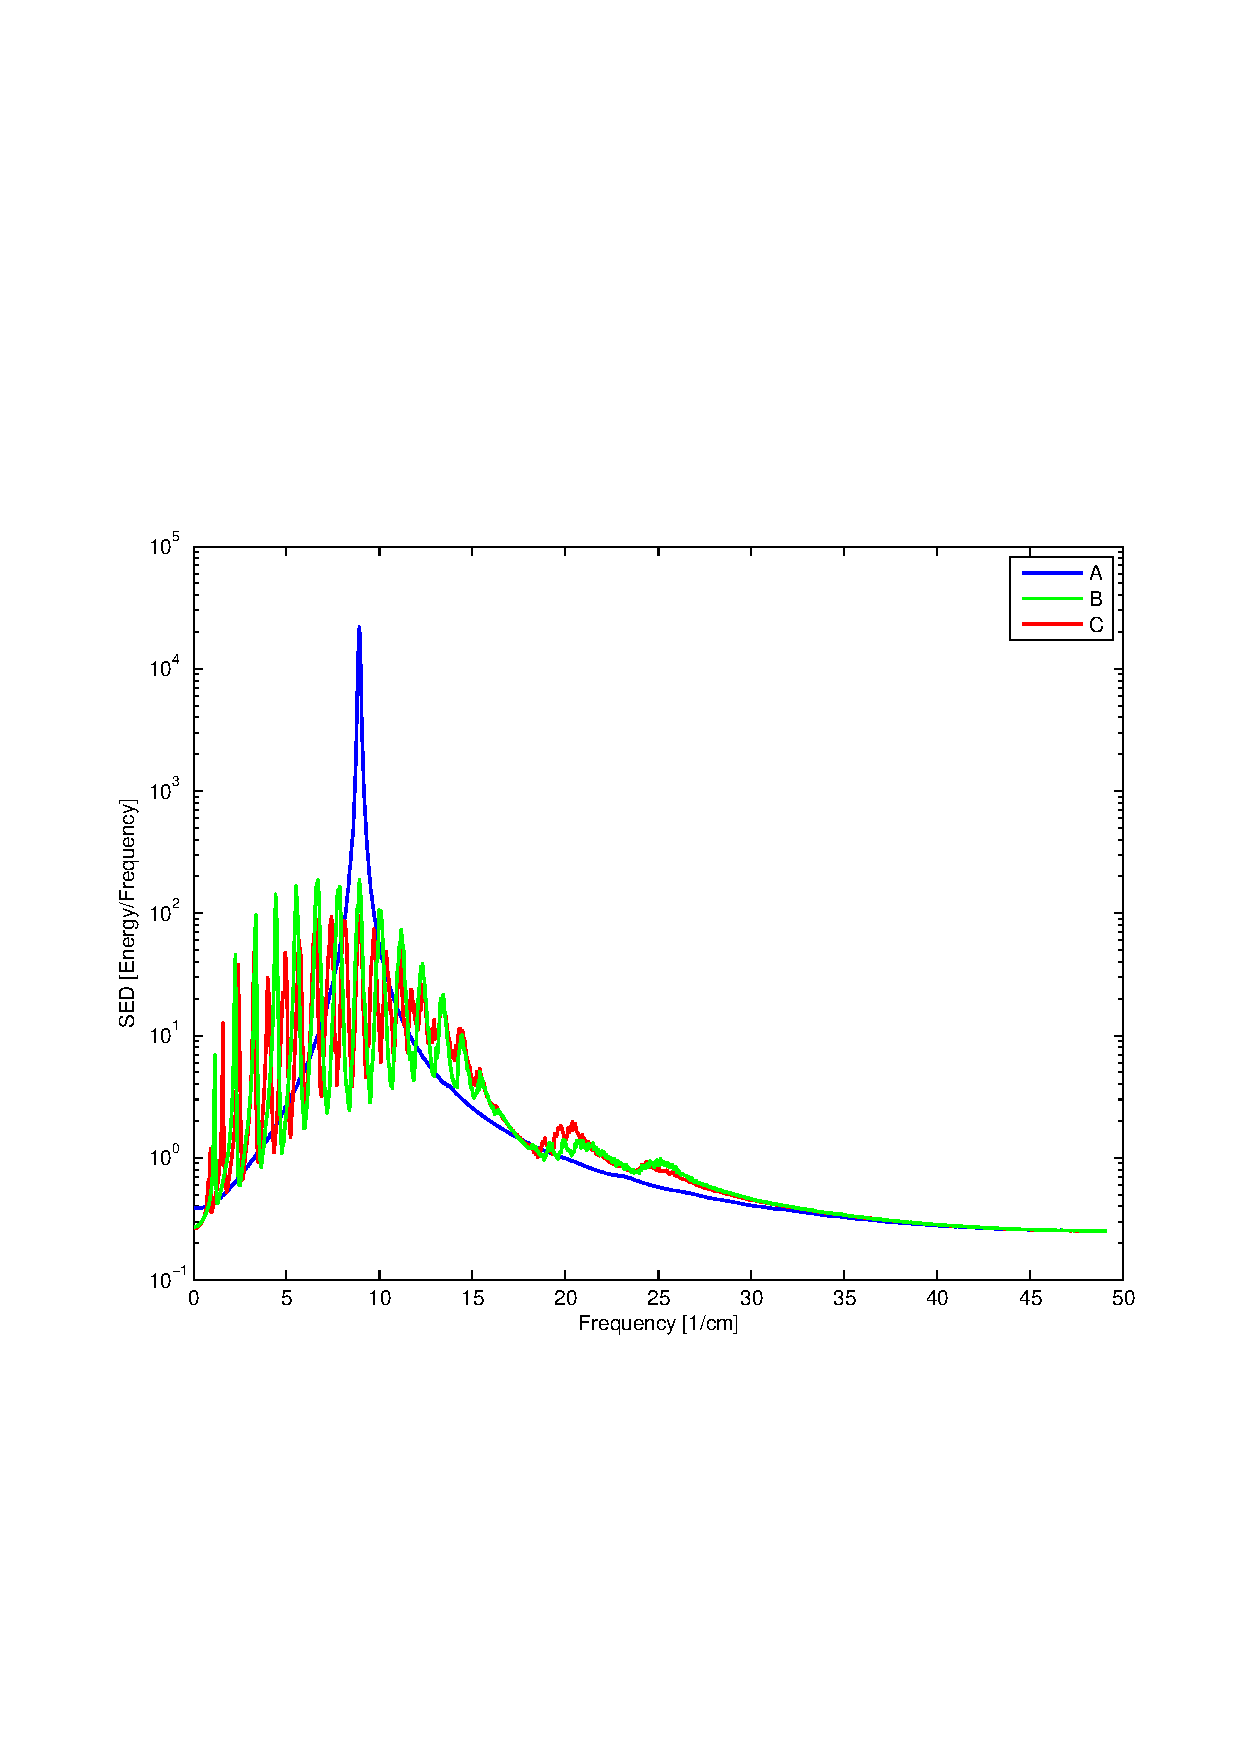
\includegraphics[scale=0.4]{peak_100_LA}
}
\end{figure}
At first glance, it is clear that the SED of Cases B and C differ from Case A. The story doesn't end there. The essence of the difference between Cases B and C and Case A lies not in the physics of the phonons, but in the model of their description. Ultimately, the idea of dividing the 32x4x4 domains into 4x4x4 blocks and performing NMD on these blocks to observe the change in the phonon lifetimes as a function of spatial position relative to the interface proved to be an ineffective approach.

The precise reason for these results is attributed to the mathematical nature of the problem. A sketch of the reason is offered here (without the formal rigour of proof). First, the definition of $Q(\pmb{\kappa},\nu)$ requires the summation over all possible $\pmb{\kappa},\nu$ of the entire 32x4x4 domain. The division into blocks discounts the entire summation to only include available $\pmb{\kappa},\nu$ of the 4x4x4 block:
\begin{eqnarray}
\begin{split}
\dot{Q}(\pmb{\kappa},\nu,t)-\frac{1}{\sqrt{N}}\sum_{28x4x4}\sqrt{m_j}exp(-i\pmb{\kappa}\cdot\pmb{r}(jl))\pmb{e}^*(j,\pmb{\kappa},\nu)\cdot\dot{\pmb{u}}(jl,t)&=\\\frac{1}{\sqrt{N}}\sum_{4x4x4}\sqrt{m_j}exp(-i\pmb{\kappa}\cdot\pmb{r}(jl))\pmb{e}^*(j,\pmb{\kappa},\nu)\cdot\dot{\pmb{u}}(jl,t).
\end{split}
\end{eqnarray}
Neglecting the modes that are uniqe to the complete 32x4x4 domain, leads to an erroneous coordinate transformation from real space, $\pmb{u}$, to k-space, ${Q}$, because of the incompleteness of the solution basis. In other words, without using all the possible modes of the system to describe the motion of an individual atom, the corresponding normal mode cannot be inferred. The reverse is equivalently true.

On a related note, the ensemble of each individual block is difficult to ascertain. The entire domain is fixed to be NVE, but the energy of a block may not be fixed with time. At any given instant the energy of one block may be more or less than one of its neighbours, but the energy of all the blocks together remains constant.

This exercise revisits the struggle to handle any deviation from the perfect periodic bulk crystal lattice. By relying on the eigenvectors and frequencies obtained from lattice dynamics, it is not obvious how to incorporates aperiodicities into this approach.

\section*{Future Steps}

The immediate challenge is to try and recover the missing information that is contained in those modes that are present, but discounted from the blocks. This is not trivial. Ultimately, one requires \textit{a priori} knowledge of the time-dependent behaviour of the normal modes. In practice, for a harmonic system, this wouldn't be difficult because the analytical solution of the normal modes is accessible given the initial conditions. For the real anharmonic system, however, this is not an alternative since there is no analytical solution.

A computationally intensive approach would be to perform NMD-SED on the entire domain, but this would not provide any information about the spatial effects of the interface upon the phonon lifetimes. It would appear that to investigate this effect requires a fundamentally different view of solids where general aperiodicities, like defects, interfaces, or surfaces can be incorporated. Perhaps the study of phonon properties in amorphous materials will offer insight into this problem.

\begin{figure}[ht]
\centering
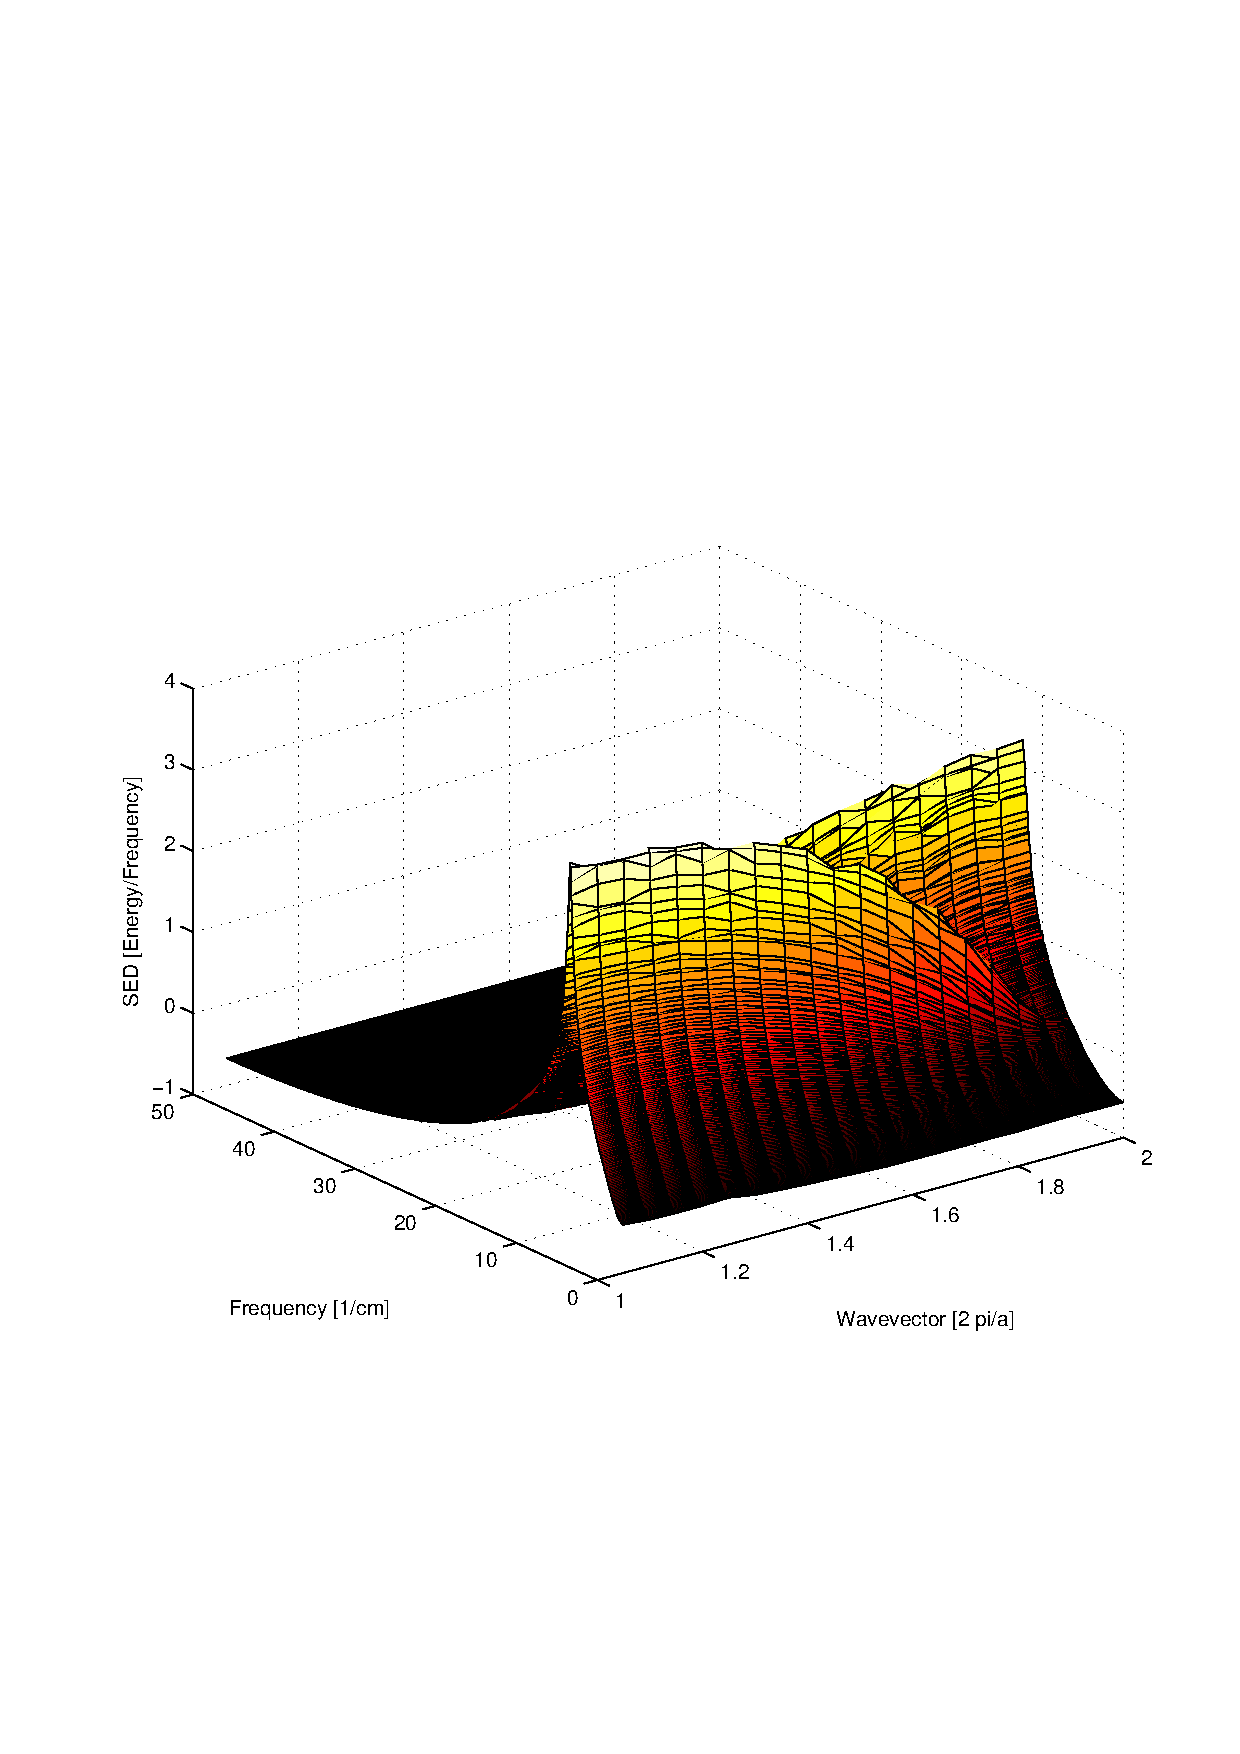
\includegraphics[scale=0.7]{spread_100_200}
\caption{Spread in $\pmb{\kappa}=[1,0,0]$ to $[2,0,0]$ }
\end{figure}

One interesting phenomenon that has yet to have a sastifactory explanation is the spread in the wavevector, as seen in Figure 3. Without proof, this result may be attributed to the anharmonicity of the crystal. At any given instant in time, the lattice constant will differ from the next and thus the definition of wavevector (or more generally, the BZ) will vary in time. If this is truly a statistical manifestion, then the spread could be quantified, analogous to the way in which the spread in frequency is measured using SED.

\newpage
\bibliographystyle{plain}
\bibliography{new.bib}
\end{document}

